\subsection{Question 2(1): Accuracy Model and Optimal Vehicle--Station Pair}\label{sec:q21}

\subsubsection{Model}

Two vehicles $i=1,2$ at stations $s_i$ observe T2 (projection $T_p$, height $H$) with
bearing errors $\varepsilon_i\sim N(0,\sigma_b^2)$, $\sigma_b=1^\circ$, independent---the
textbook bearings-only measurement model \cite{torrieri1984,kay1993}:
\begin{equation}\label{eq:meas}
\phi_i=\operatorname{atan2}\bigl(T_y-s_{iy},\,T_x-s_{ix}\bigr)+\varepsilon_i .
\end{equation}
Linearizing Eq.~\eqref{eq:meas} at the true position, each bearing constrains the
position along the unit normal $n_i$ of its sightline, with sensitivity $1/d_i$ where
$d_i=\|s_i-T_p\|$:
\begin{equation}\label{eq:fisher}
I=\sigma_b^{-2}\sum_{i=1}^{2}\frac{n_i n_i^{\mathsf T}}{d_i^{2}},\qquad
C=I^{-1} .
\end{equation}
For the $2\times2$ Gram matrix $G=\sum_i n_i n_i^{\mathsf T}/d_i^2$ one has
$\operatorname{tr}G=d_1^{-2}+d_2^{-2}$ and $\det G=\sin^2\gamma/(d_1^2d_2^2)$, where
$\gamma$ is the crossing angle of the two sightlines; hence
\begin{equation}\label{eq:rmse}
\operatorname{tr}C=\frac{\operatorname{tr}G}{\det G}\,\sigma_b^{2}
=\sigma_b^{2}\,\frac{d_1^{2}+d_2^{2}}{\sin^{2}\gamma},
\qquad
\mathrm{RMSE}=\sqrt{\operatorname{tr}C}
=\sigma_b\,\frac{\sqrt{d_1^{2}+d_2^{2}}}{\sin\gamma}.
\end{equation}
Equation~\eqref{eq:rmse} is the requested accuracy law in one line: the baseline $B$
acts through the geometry linking $(d_1,d_2,\gamma)$
($B^2=d_1^2+d_2^2-2d_1d_2\cos\gamma$), the crossing angle enters as $1/\sin\gamma$.
Elevation Eq.~\eqref{eq:elev} forces $d_i\ge r_{80}=5.8188\,\mathrm{m}$ for T2, so
\begin{equation}\label{eq:lb}
\mathrm{RMSE}\;\ge\;\sigma_b\sqrt{2}\;r_{80}=0.14362\,\mathrm{m},
\end{equation}
with equality \emph{iff} $\gamma=90^\circ$ and $d_1=d_2=r_{80}$: both stations on the
$r_{80}$-circle, separated by a $90^\circ$ arc as seen from the target (perpendicular
sightlines). Under the hard operating margins of Assumption~7 (clearance
$\ge0.10\,\mathrm{m}$ beyond the $1.5$-m buffer, elevation $\le79.9^\circ$), the
smallest admissible radius is $r_{80}+0.10\,\mathrm{m}=5.9188\,\mathrm{m}$, so the
margin-compliant optimum is
$\sigma_b\sqrt2\,(r_{80}+0.10)=0.146092\,\mathrm{m}$---$1.73\%$ above the bound;
relaxing the margins to zero recovers Eq.~\eqref{eq:lb} exactly. We adopt
$\mathrm{RMSE}=\sqrt{\operatorname{tr}C}$ (A-optimality, meters) as primary metric: it
is proportional to $\sigma_b$, so the optimal pair is independent of $\sigma_b$;
$\det C$ (D-optimality) and $\operatorname{cond}C$ are secondary diagnostics.

Feasibility: station $s_i$ must lie in $\mathcal{F}_{T_2}\cap\mathcal{R}_i$, where
$\mathcal{R}_i$ is the $90$-m geodesic disc of vehicle $i$ (30\,s $\times$
$3\,\mathrm{m}/\mathrm{s}$, Assumption~2). The optimization is
\begin{equation}\label{eq:q21opt}
\min_{\{i,j\}\subset\{1..5\}}\;\min_{s_i\in\mathcal{F}_{T_2}\cap\mathcal{R}_i,\;
s_j\in\mathcal{F}_{T_2}\cap\mathcal{R}_j}\;
\sigma_b\frac{\sqrt{d_i^{2}+d_j^{2}}}{\sin\gamma(s_i,s_j)} .
\end{equation}

\subsubsection{Algorithm}

Outer layer: all $\binom{5}{2}=10$ vehicle pairs. Inner layer, per pair: a
hard-constrained scan of the analytic $90^\circ$ family---stations at target-azimuth
$\phi$ and $\phi+90^\circ$ (perpendicular sightlines; a $\phi+180^\circ$ pair would be
collinear and degenerate) on the operating circles
$r\in\{r_{80}+0.10,\,+0.12,\,+0.15,\,+0.20\}\,\mathrm{m}$---with the Assumption~7
margins enforced (clearance $\ge0.10\,\mathrm{m}$ beyond the buffer, elevation
$\le79.9^\circ$), $\phi$ scanned at $0.1^\circ$ and refined locally at
$0.005^\circ$/$0.002\,\mathrm{m}$; for each $\phi$ both assignments of the two
stations to $\{V_i,V_j\}$ are evaluated, and every candidate must satisfy travel
$\le30\,\mathrm{s}$ on visibility-graph paths (Fig.~\ref{fig:q2reach}). Ties in
RMSE---at the $1$-mm reporting granularity every margin-compliant radius in the band
rounds to the same value---are broken by the declared secondary criterion: the
two-vehicle \emph{mission-completion time}
$\max_i(t_i+\tau_i)+5+\max_i(\tau_i)$ (consistent with Q1's rule and the problem's
rapid-deployment objective), then total travel, then midpoint distance to $O$, then
azimuth. Pairs whose family scan is infeasible everywhere under the margins are
marked infeasible.

\begin{figure}[!htb]\centering
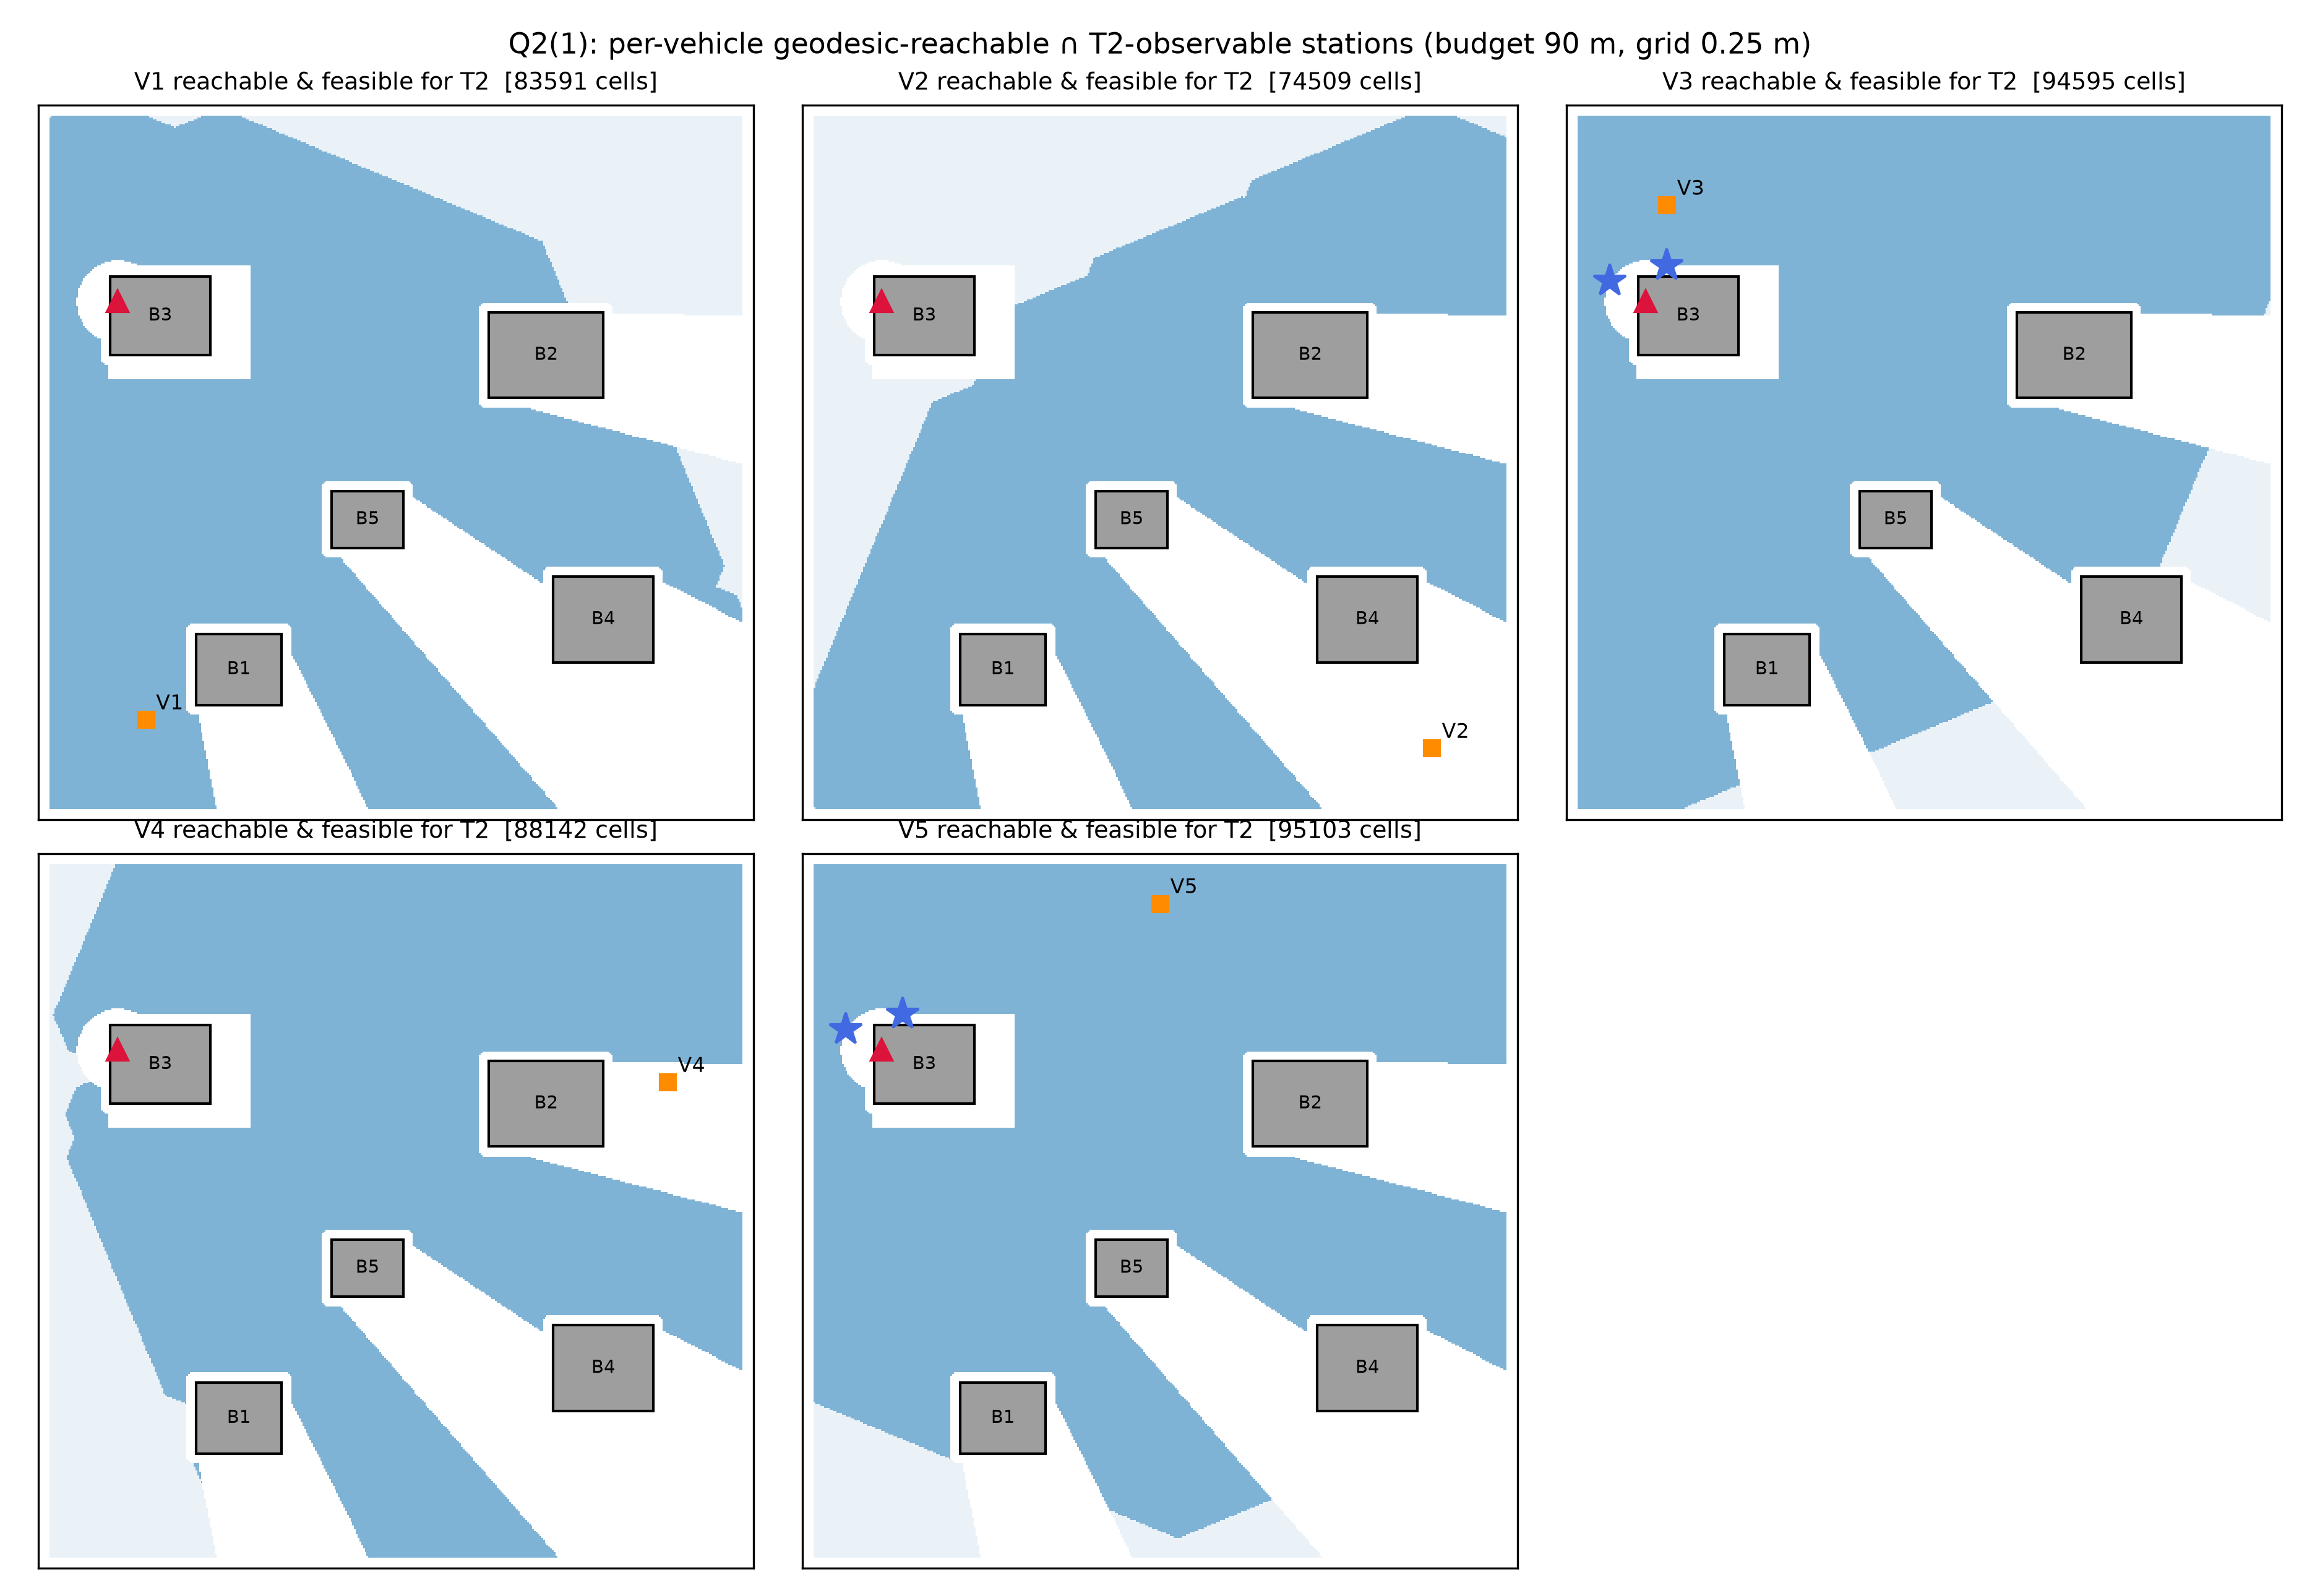
\includegraphics[width=0.55\textwidth]{fig_q2_1_reachability.png}
\caption{Reachable sets ($\le90$-m geodesic) intersected with $\mathcal{F}_{T_2}$ for the
five vehicles. V2's intersection is by far the poorest, foreshadowing its exclusion from
every competitive pair.}
\label{fig:q2reach}
\end{figure}

\subsubsection{Results}

\begin{table}[!htb]\centering\small
\setlength{\tabcolsep}{4.5pt}
\caption{Margin-compliant optimum by vehicle pair ($r=r_{80}+0.10$ m,
$\gamma=90^\circ$ and $B=8.370$ m for every pair; travels within the 30-s budget).
V2-containing pairs have no margin-compliant candidate within the budget and are
omitted.}
\label{tab:q21pairs}
\begin{tabular}{ccccc}
\toprule
Pair & RMSE (m) & $r$ (m) & total travel (s) & mission (s) \\
\midrule
(3,5) & 0.14609 & 5.9188 & 19.88 & 24.53 \\
(1,3) & 0.14609 & 5.9188 & 22.43 & 28.20 \\
(1,5) & 0.14609 & 5.9188 & 33.86 & 28.20 \\
(3,4) & 0.14609 & 5.9188 & 32.17 & 36.83 \\
(4,5) & 0.14609 & 5.9188 & 43.57 & 36.83 \\
(1,4) & 0.14609 & 5.9188 & 45.93 & 36.83 \\
\bottomrule
\end{tabular}
\end{table}

Table~\ref{tab:q21pairs} shows the same stratification as the unconstrained scan:
every pair excluding V2 reaches the margin-compliant optimum
$0.14609\,\mathrm{m}$ ($+1.73\%$ over the bound), while the four V2-containing pairs
have \emph{no} margin-compliant candidate within the travel budget at all---their
reachable intersection with $\mathcal{F}_{T_2}$ (Fig.~\ref{fig:q2reach}) is the
poorest, and under the unconstrained scan they stagnated near $0.30\,\mathrm{m}$
($2.1\times$ the bound). The mission-time tie-break selects \textbf{V3+V5}
(mission $24.53\,\mathrm{s}$ vs.\ $28.20$--$36.83\,\mathrm{s}$ for the other five);
the chosen five-fold output is consolidated in Table~\ref{tab:q21chosen}:

\begin{table}[!htb]\centering\small
\caption{Required five-fold output for the chosen vehicle--station pair.}
\label{tab:q21chosen}
\begin{tabular}{lc}
\toprule
Quantity & Value \\
\midrule
Vehicle pair & V3 $+$ V5 \\
Station of V3 / travel & $(5.203609,\;71.451873)$ / $5.667\,\mathrm{s}$ ($17.00\,\mathrm{m}$) \\
Station of V5 / travel & $(9.980729,\;78.325247)$ / $14.208\,\mathrm{s}$ ($42.62\,\mathrm{m}$) \\
Baseline $B$ / crossing angle $\gamma$ & $8.3704\,\mathrm{m}$ / $90.00^\circ$ \\
RMSE $=\sqrt{\operatorname{tr}C}$ & $0.146092\,\mathrm{m}$ ($+1.73\%$ over the margin-free bound) \\
$\det C$ / condition number & $1.139\times10^{-4}\,\mathrm{m}^4$ / $1.000$ \\
$1\sigma$ error-ellipse axes & $0.10330\,\mathrm{m}$ (isotropic) \\
$\mathrm{CEP}_{50}$ & $0.1216\,\mathrm{m}$ (Rayleigh) \\
Operating margins & clearance $3.30/0.83\,\mathrm{m}$ beyond buffer; elevation $79.83^\circ$ \\
Observation start / mission completion & $16.869\,\mathrm{s}$ / $24.530\,\mathrm{s}$ \\
\bottomrule
\end{tabular}
\end{table}

\begin{figure}[!htb]\centering
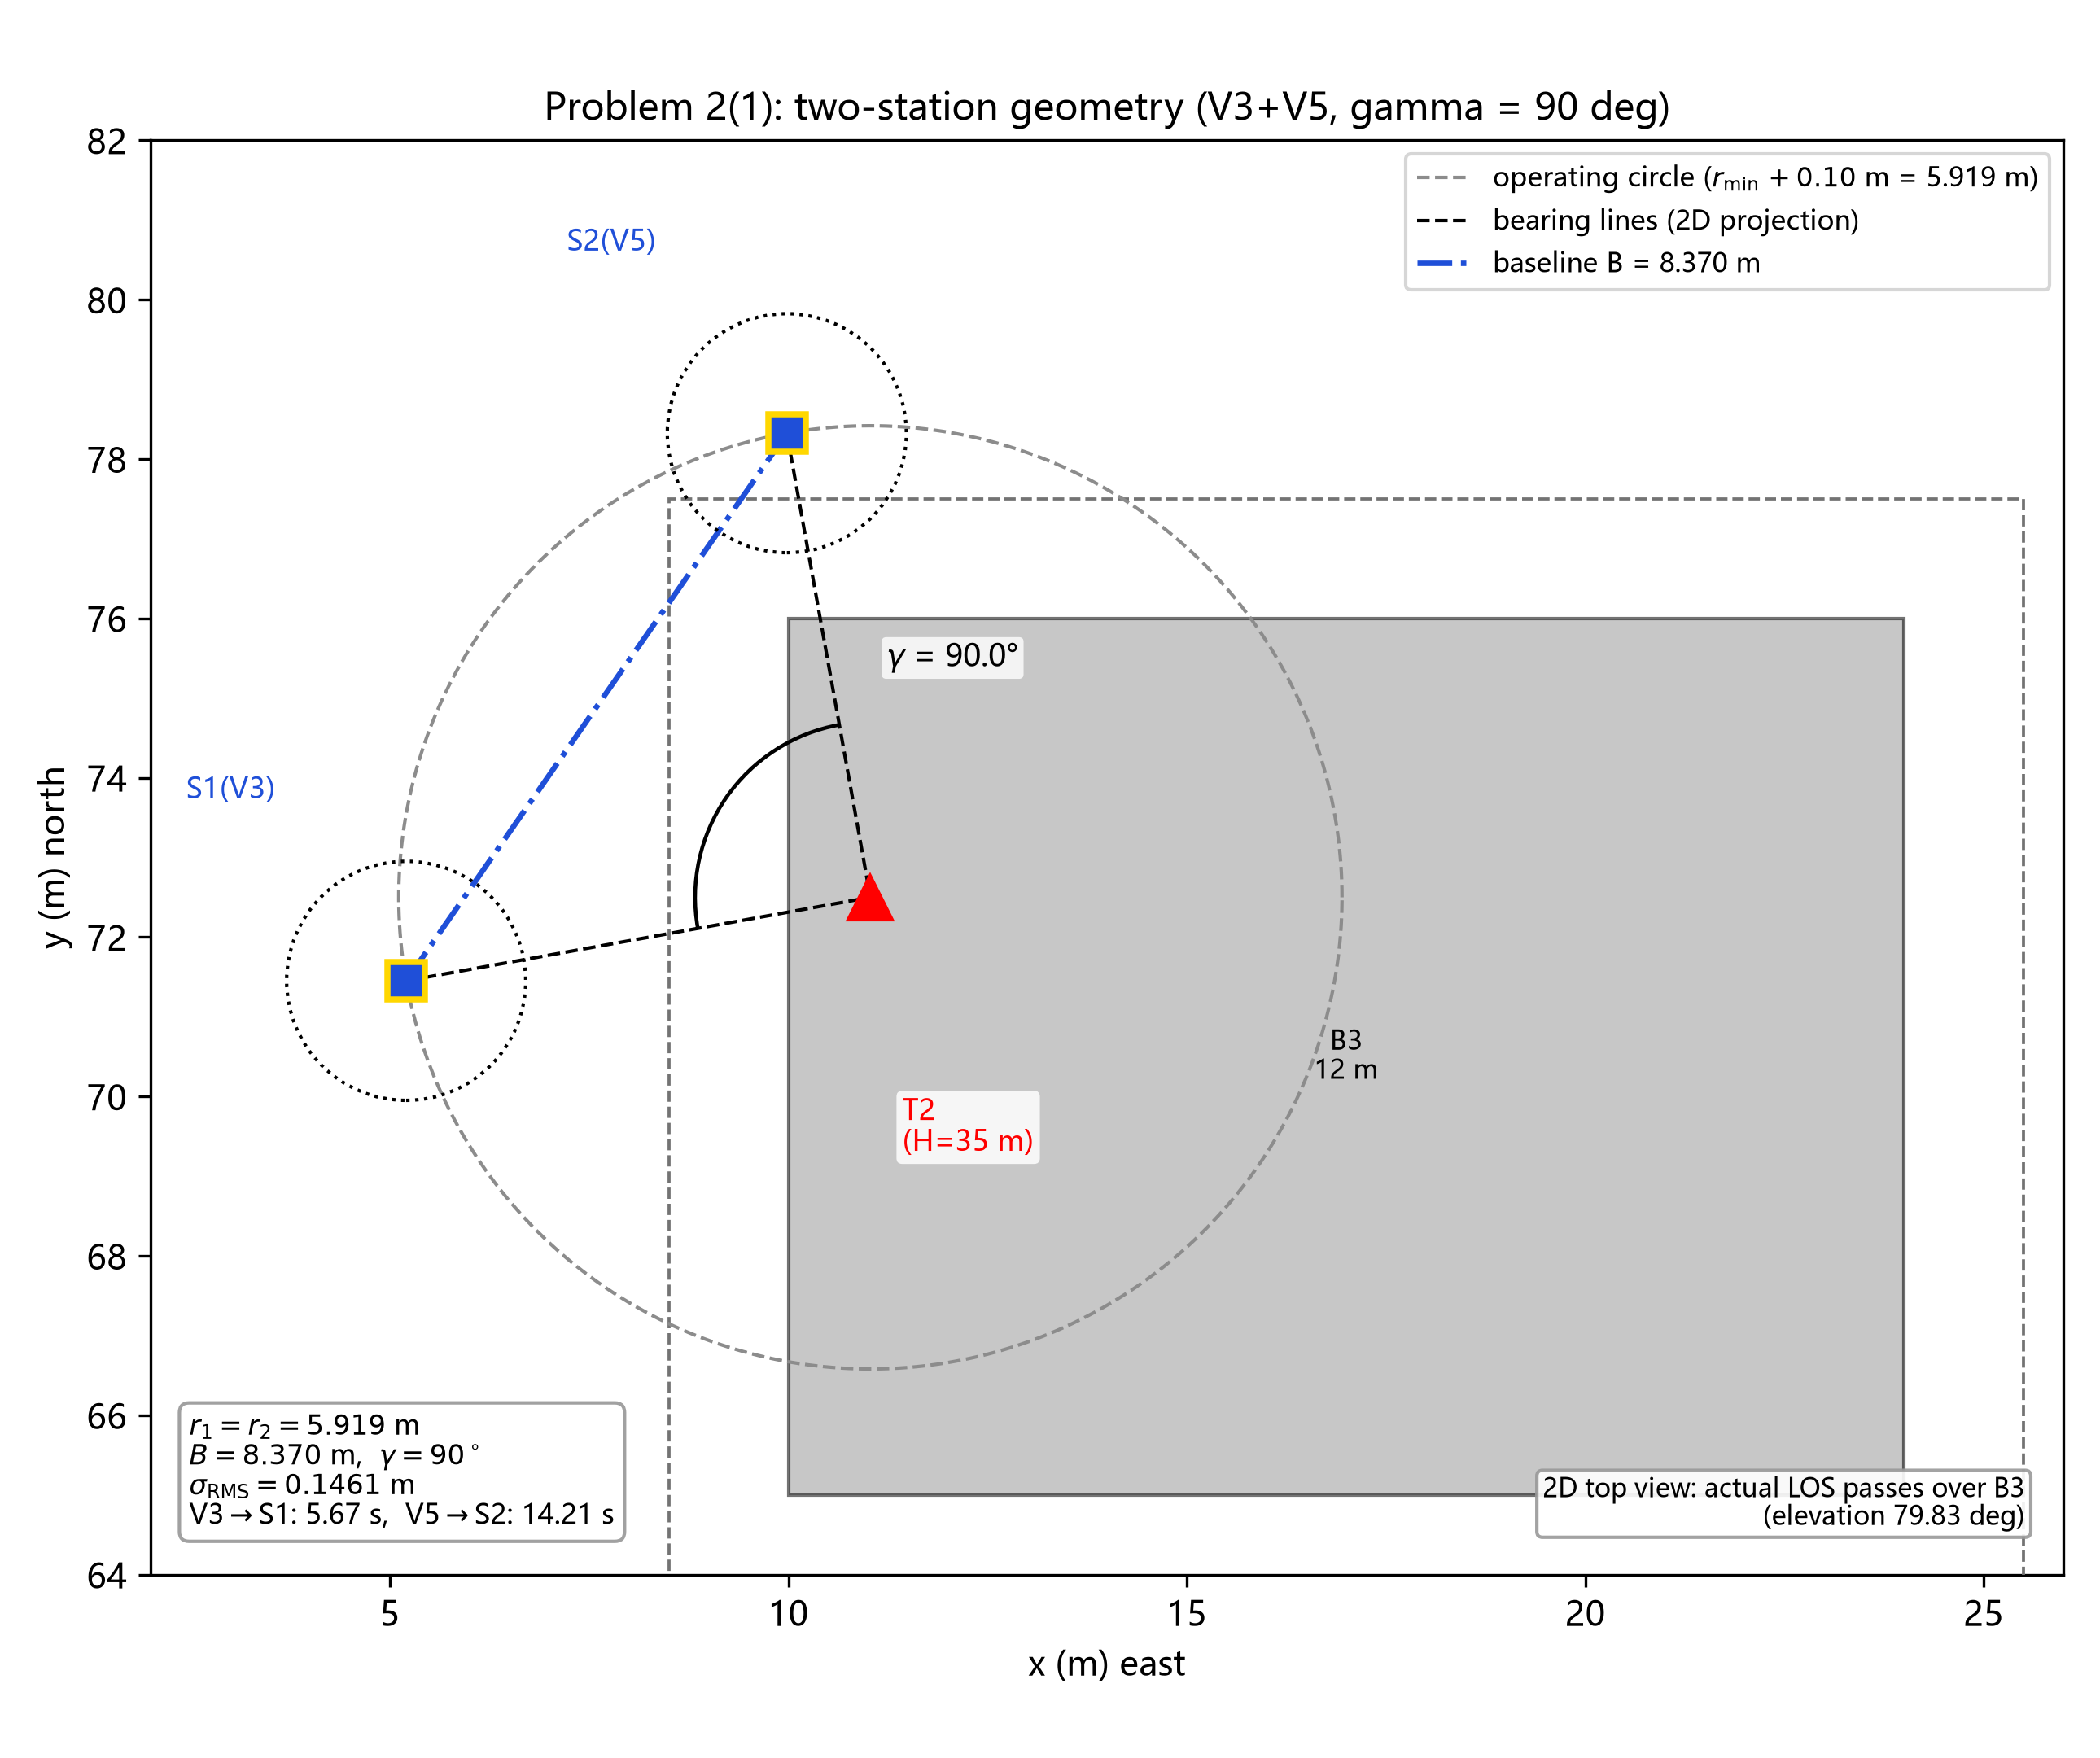
\includegraphics[width=0.6\textwidth]{fig_q2_1_geometry.png}
\caption{Margin-compliant two-station geometry for T2 (V3+V5, $\gamma=90^\circ$,
$r=r_{80}+0.10\,\mathrm{m}$): both stations sit outside the $1.5$-m vehicle buffer
(dashed) with the Assumption-7 margins built in; the horizontal projections of the
sightlines pass over $B_3$ (the actual LOS clears the roof at elevation
$79.83^\circ$, minimum prism distance $0.55\,\mathrm{m}$).}
\label{fig:q2geom}
\end{figure}

The conditional covariance $C$ is \emph{isotropic} ($\operatorname{cond}C=1.000$,
circular $1\sigma$ ellipse of radius $0.1033$ m): at $\gamma=90^\circ$ with equal
distances the two bearing constraints are orthogonal---precisely the geometric meaning
of the bound. The isotropic Gaussian also fixes the operational metric: the radial
error is Rayleigh with median $\mathrm{CEP}_{50}=\sigma_{1D}\sqrt{2\ln2}=0.1216\,\mathrm{m}$
---half of all fixes land within $12$ cm. Both deployed stations carry the declared
margins: elevations $79.83^\circ$ ($0.17^\circ$ below the limit), clearances
$3.30/0.83\,\mathrm{m}$ beyond the buffer, and LOS minimum distances
$2.99/0.55\,\mathrm{m}$ from the nearest prism---the insurance recommended by the
degeneracy discussion is built into the reported deployment.

\textbf{Degenerate configurations.} Equation~\eqref{eq:rmse} quantifies the two
degeneracies the problem asks about. As $\gamma\to0^\circ$ or $180^\circ$,
$\mathrm{RMSE}\propto1/\sin\gamma$ diverges: the two sightlines become parallel, the
position along the baseline direction is unconstrained, $\operatorname{cond}C\to\infty$
and the error ellipse degenerates into a strip (Fig.~\ref{fig:q2gamma}a). The adopted
mitigation is an azimuth guard $\gamma\ge1^\circ$ (hard feasibility) plus an operating
recommendation of $30^\circ\le\gamma\le150^\circ$ read off the sweep. Stations at
region-boundary tangency are handled by the closed-set convention; a margin of
$\delta$ m costs at most $O(\delta)$ in $d_i$. Concretely, the \emph{adopted}
$0.10$-m radial offset keeps $\gamma=90^\circ$, buys $0.17^\circ$ of elevation slack
and $0.83$--$3.30\,\mathrm{m}$ of clearance beyond the buffer, and costs $1.73\%$
RMSE ($0.1461$ vs $0.14362\,\mathrm{m}$)---cheap insurance, built into the reported
deployment rather than left as advice (Section~\ref{sec:sens}).

\begin{figure}[!htb]\centering
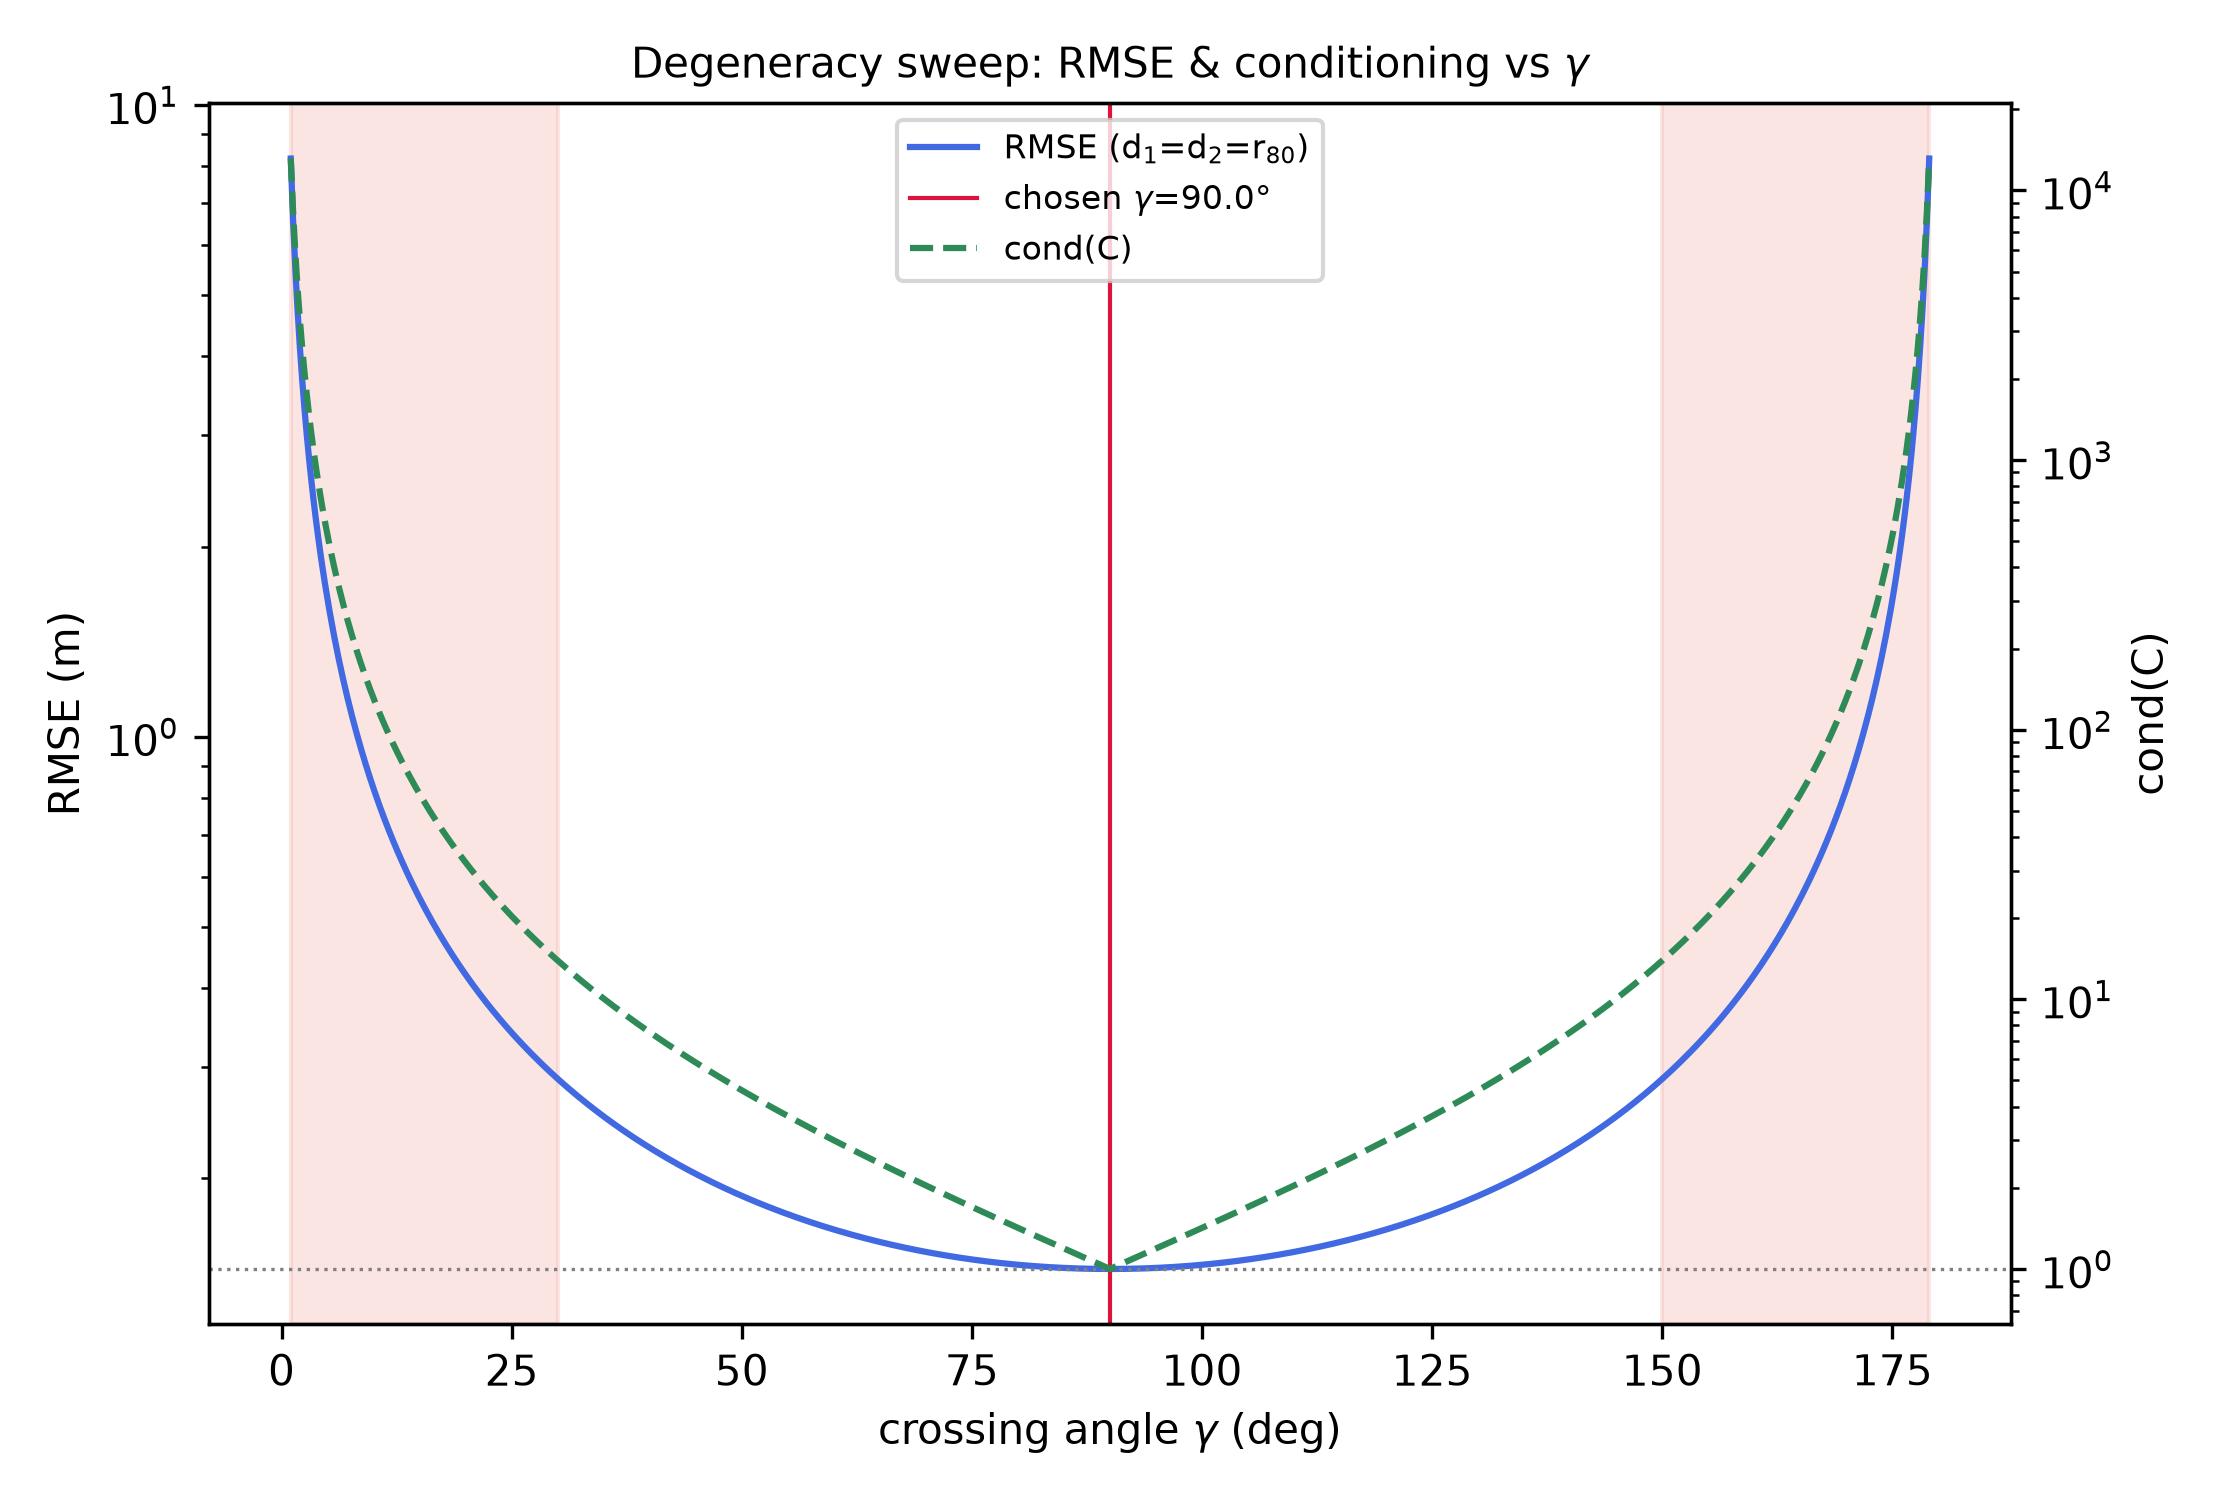
\includegraphics[width=0.46\textwidth]{fig_q2_1_gamma_degeneracy.png}\hfill
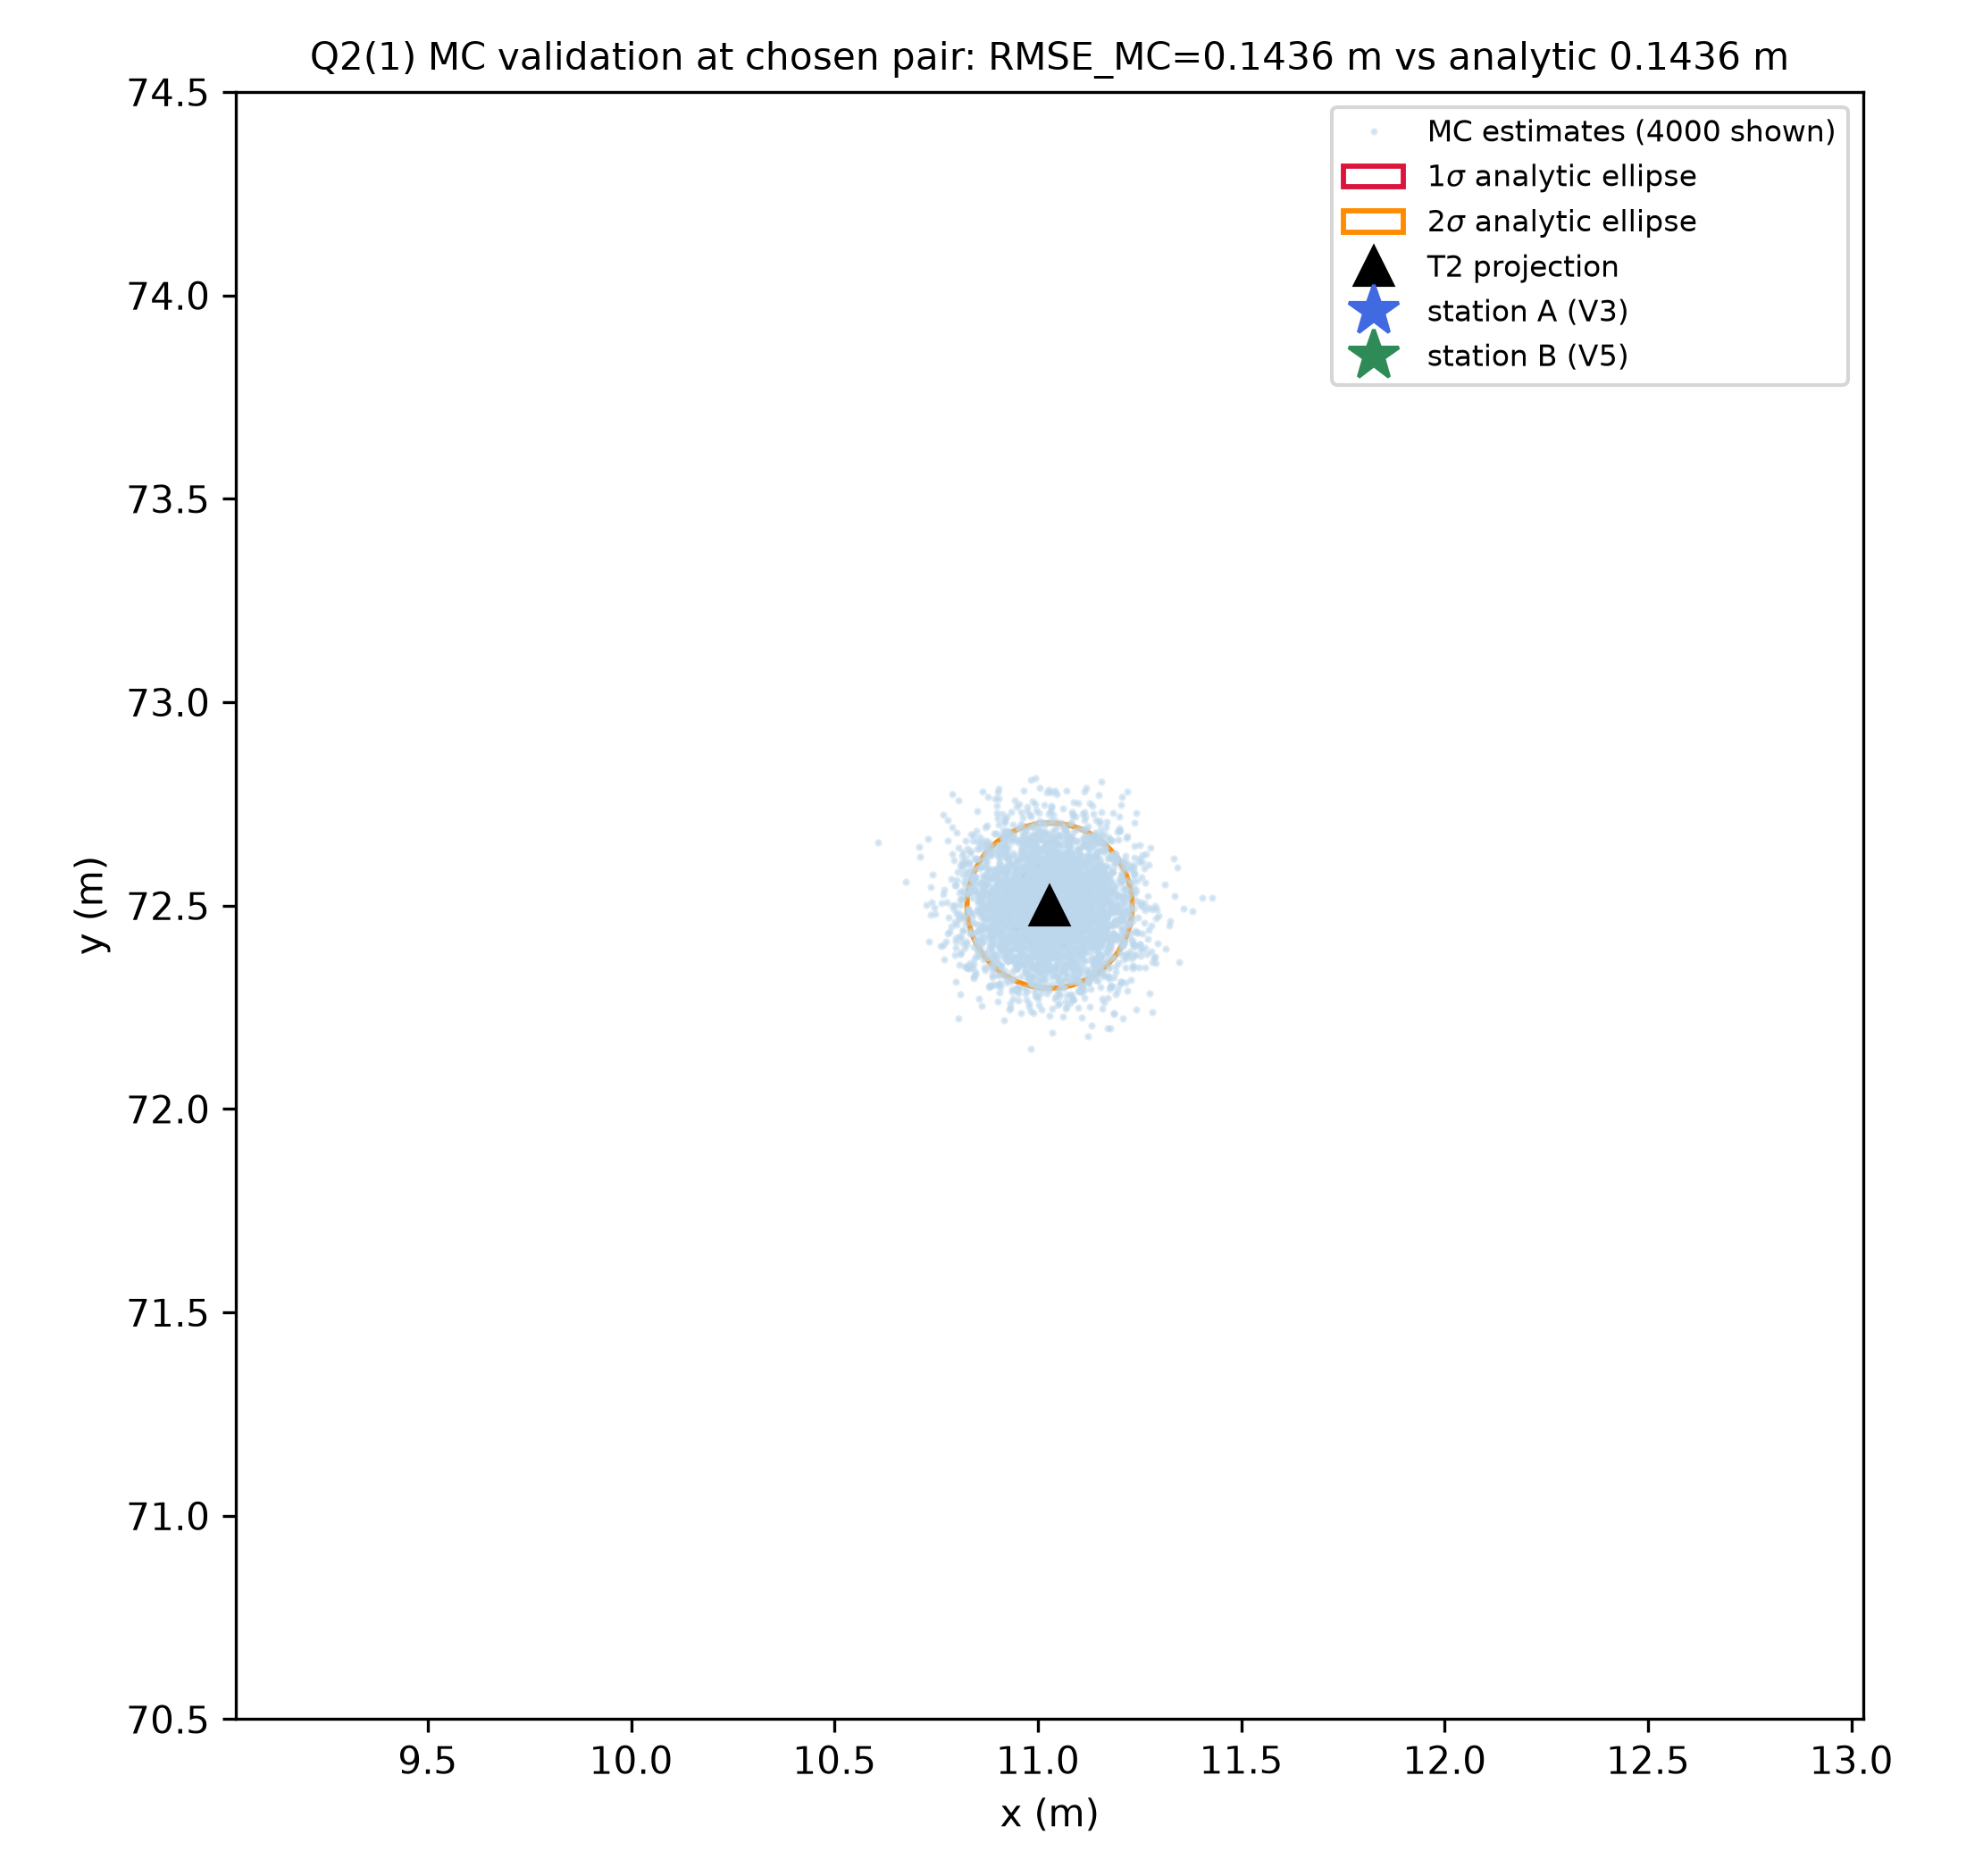
\includegraphics[width=0.46\textwidth]{fig_q2_1_mc_validation.png}
\caption{(a) Degeneracy sweep: RMSE ($\propto1/\sin\gamma$) and $\operatorname{cond}C$
explode as the crossing angle approaches $0^\circ$ or $180^\circ$; the flat band around
$90^\circ$ is operationally safe. (b) Monte Carlo validation ($2\times10^{5}$ samples):
the empirical error scatter (round red) is isotropic with empirical RMSE $0.14363$ m,
matching the analytic covariance ellipse of Eq.~\eqref{eq:fisher} (blue).}
\label{fig:q2gamma}
\end{figure}

\subsubsection{Validation}

A Monte Carlo experiment with $2\times10^{5}$ samples (sampling the two bearing errors,
intersecting the two bearing lines exactly) at the bound geometry yields empirical
RMSE $=0.14363\,\mathrm{m}$ against the analytic $0.14362\,\mathrm{m}$---relative
deviation $0.0\%$ (Fig.~\ref{fig:q2gamma}b); the estimate's Monte-Carlo standard
error, $\mathrm{RMSE}/\sqrt{2N}=2.3\times10^{-4}\,\mathrm{m}$ ($0.16\%$), bounds the
deviation to within one standard error, and the experiment repeats unchanged at the
deployed margin-compliant geometry (all distances scale by $+1.73\%$). The 30-s
travel feasibility of both deployed stations was re-checked on the visibility graph
($17.00$ m and $42.62$ m, well within $90$ m), both stations were re-verified inside
$\mathcal{F}_{T_2}$ by the Q1 solver with the Assumption-7 margins, and the LOS
minimum prism distances ($2.99/0.55\,\mathrm{m}$) certify clearance. Finally,
because $C\propto\sigma_b^2$, re-running the optimization with
$\sigma_b\in\{0.5^\circ,1^\circ,2^\circ\}$ rescales every pair's RMSE proportionally
($0.07301/0.14609/0.29219\,\mathrm{m}$ at the chosen pair) and leaves the argmin unchanged: the
station-pair selection is structurally independent of the bearing-error magnitude.
\emph{Conclusion: the analytic model and the empirical estimator agree to within
Monte Carlo noise, the selected pair is optimal for every $\sigma_b$, and the
deployed margins are verified rather than assumed.}
